% Tento soubor nahraďte vlastním souborem s přílohami (nadpisy níže jsou pouze pro příklad)

\chapter{Inštalácia a spustenie aplikácie} \label{sec:instalacia}
  Aplikácia je určená ako voľne distribuovateľná spolu so zdrojovými súbormi. Prerekvizitami aplikácie sú Python~3 a príslušný správca balíčkov \texttt{pip},
  pomocou ktorých je možné doinštalovať všetky potrebné balíčky. Tieto balíčky sú uvedené v súbore \texttt{requirements.txt}. Pred inštaláciou odporúčam
  vytvoriť virtuálne prostredie pre Python pomocou modulu \texttt{venv}. Odporúčaný postup inštalácie je nasledovný:
  \begin{enumerate}
    \item Vytvorenie virtuálneho prostredia \texttt{venv} pomocou príkazu \texttt{python3 -m venv <cesta pre novy priecinok prostredia>}.
    \item Aktivácia prostredia pomocou skriptu \texttt{cesta/k/venv/bin/activate}. Na sytémoch Windows je táto cesta \texttt{cesta/k/venv/Scripts/activate}.
    \item Inštalácia balíčkov pomocou príkazu \texttt{python -m pip install -r requirements.txt}.
  \end{enumerate}
  Na systémoch \emph{Linux} a \emph{macOS} sa tieto príkazy vykonávajú v príkazovom riadku terminálu. Na systémoch \emph{Windows} v prostredí PowerShell.
  Využitie virtuálneho prostredia je plne voliteľné a je sem zahrnuté ako možnosť pre prípad, že užívateľ nechce nainštalovať potrebné balíčky do systémovej
  verzie Python\footnote{Po odstránení priečinku virtuálneho prostredia sa vymažú všetky v rámci neho inštalované balíčky.}.

  Aplikácia sa vo virtuálnom prostredí spúšťa príkazom \texttt{python app.py}.

\chapter{Názvy súborov použitých pre testovanie klasifikácie} \label{priloha:zoznam_suborov}
  \begin{table}[ht]
    \centering
    \caption{Tabuľka súborov použitých pre vyhodnotenie automatickej klasifikácie. Skratky tried sú: O - oblúk, KO - klenutý oblúk,
    ĽS - ľavá slučka, PS - pravá sľučka, Š / DS - špirála / dvojitá slučka.}
    \begin{tabular}{ | c | c | c | }
      \hline
      \multicolumn{3}{|c|}{Triedy odtlačkov}            \\
      \hline
      O       & KO        & ĽS \\
      \hline
      1143\_1\_1\_L2.bmp & 1184\_1\_3\_L2.bmp & 1101\_1\_1\_L2.bmp  \\
      1143\_1\_2\_P2.bmp & 1184\_2\_3\_L2.bmp & 1101\_2\_1\_L2.bmp  \\
      1143\_2\_1\_P2.bmp & 1284\_1\_1\_L4.bmp & 1115\_1\_2\_L3.bmp  \\
      1143\_2\_3\_L2.bmp & 1284\_1\_3\_P2.bmp & 1213\_2\_2\_L2.bmp  \\
      1143\_1\_1\_L3.bmp & 1184\_2\_1\_L2.bmp & 1213\_1\_1\_L3.bmp  \\
      1143\_1\_2\_P3.bmp & 1184\_3\_1\_L2.bmp & 1101\_2\_2\_L5.bmp  \\
      1143\_2\_1\_P3.bmp & 1284\_1\_1\_P2.bmp & 1115\_1\_3\_L3.bmp  \\
      1143\_2\_3\_P2.bmp & 1284\_3\_3\_P2.bmp & 1265\_1\_1\_L2.bmp  \\
      1143\_1\_1\_P2.bmp & 1184\_2\_2\_L2.bmp & 1101\_1\_2\_L2.bmp  \\
      1143\_1\_3\_L2.bmp & 1184\_3\_2\_L2.bmp & 1213\_1\_1\_L5.bmp  \\
      1143\_2\_2\_L2.bmp & 1284\_1\_2\_L4.bmp & 1115\_2\_1\_L2.bmp  \\
      1284\_3\_3\_L1.bmp &                 & 1284\_1\_1\_L1.bmp     \\
      1143\_1\_1\_P3.bmp &                 & 1101\_1\_2\_L3.bmp     \\
      1143\_1\_3\_L3.bmp &                 & 1101\_2\_3\_L5.bmp     \\
      1143\_2\_2\_L3.bmp &                 & 1115\_2\_1\_L3.bmp     \\
      1143\_1\_2\_L2.bmp &                 & 1101\_1\_2\_L5.bmp     \\
      1143\_1\_3\_P2.bmp &                 & 1115\_1\_1\_L2.bmp     \\
      1143\_2\_2\_P2.bmp &                 & 1115\_2\_2\_L3.bmp     \\
      1143\_1\_2\_L3.bmp &                 & 1101\_1\_3\_L2.bmp     \\
      1143\_1\_3\_P3.bmp &                 & 1115\_1\_1\_L3.bmp     \\
      1143\_2\_2\_P3.bmp &                 & 1115\_2\_3\_L3.bmp     \\
                      &                 & 1115\_1\_2\_L2.bmp        \\
                      &                 & 1213\_1\_3\_L5.bmp        \\
      \hline
    \end{tabular}
    \label{tab:subory_testov}
  \end{table}

  \begin{table}
    \centering
    \caption{Pokračovanie tabuľky \ref{tab:subory_testov}.}
    \begin{tabular}{ | c | c | }
      \hline
      \multicolumn{2}{|c|}{Triedy odtlačkov}            \\
      \hline
      PS    & Š / DS     \\
      \hline
       1101\_1\_1\_P3.bmp & 1101\_2\_1\_L4.bmp \\
       1184\_1\_2\_P3.bmp & 1115\_1\_3\_P5.bmp \\
       1115\_2\_1\_P4.bmp & 1115\_2\_3\_P5.bmp \\
       1265\_1\_3\_P3.bmp & 1253\_1\_1\_P5.bmp \\
       1101\_1\_2\_P3.bmp & 1115\_1\_1\_L4.bmp \\
       1115\_1\_2\_P3.bmp & 1115\_2\_1\_L4.bmp \\
       1115\_2\_2\_P3.bmp & 1115\_3\_1\_L4.bmp \\
       1284\_1\_2\_P3.bmp & 1253\_2\_1\_P2.bmp \\
       1101\_1\_3\_P3.bmp & 1115\_1\_1\_L5.bmp \\
       1115\_1\_2\_P4.bmp & 1115\_2\_1\_L5.bmp \\
       1115\_2\_2\_P4.bmp & 1213\_3\_1\_P2.bmp \\
       1284\_1\_2\_P4.bmp & 1253\_2\_1\_P5.bmp \\
       1101\_2\_1\_P2.bmp & 1115\_1\_1\_P5.bmp \\
       1184\_1\_3\_P2.bmp & 1115\_2\_1\_P5.bmp \\
       1115\_2\_3\_P3.bmp & 1213\_3\_2\_P2.bmp \\
       1284\_1\_2\_P5.bmp & 1253\_3\_1\_P4.bmp \\
       1115\_1\_3\_P3.bmp & 1115\_2\_2\_L4.bmp \\
       1115\_2\_3\_P4.bmp & 1213\_3\_2\_P4.bmp \\
       1115\_1\_1\_P3.bmp & 1253\_3\_1\_P5.bmp \\
       1115\_1\_3\_P4.bmp & 1115\_1\_2\_L5.bmp \\
       1115\_3\_2\_P3.bmp & 1115\_2\_2\_L5.bmp \\
       1115\_1\_1\_P4.bmp & 1213\_3\_3\_P2.bmp \\
       1115\_2\_1\_P3.bmp & 1115\_1\_2\_P5.bmp \\
       1233\_1\_3\_P3.bmp & 1115\_2\_2\_P5.bmp \\
                          & 1213\_3\_3\_P4.bmp \\
                          & 1115\_1\_3\_L4.bmp \\
                          & 1115\_2\_3\_L4.bmp \\
                          & 1233\_1\_3\_P2.bmp \\
                          & 1115\_1\_3\_L5.bmp \\
                          & 1115\_2\_3\_L5.bmp \\
                          & 1233\_3\_3\_P1.bmp  \\
                          & 1115\_1\_2\_L4.bmp \\
      \hline
    \end{tabular}
  \end{table}

\chapter{Výsledky krokov spracovania snímok z rôznych snímačov} \label{priloha:vysledky_spracovania}
  V tejto prílohe sú zobrazené niektoré kroky spracovania vstupných snímok z rôznych snímačov. Snímky pochádzajú z toho istého prsta pri každom snímači.
  Zoradenie je pri každom obrázku rovnaké, a to nasledovné:
  \begin{itemize}
    \item Prvý riadok, zľava doprava: originálna snímka, lokálne frekvencie, orientácie.
    \item Druhý riadok, zľava doprava: Gaborovo filtrovanie s následnou binarizáciou, stenčenie línií, singularity.
  \end{itemize}

  \begin{figure*}[h]\centering
    \centering
    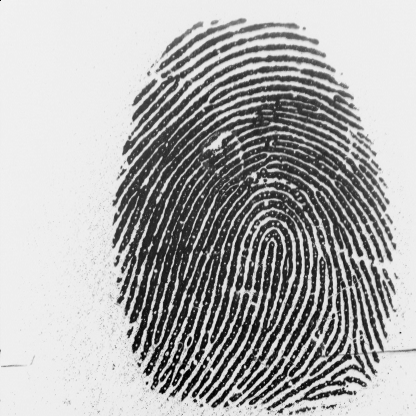
\includegraphics[width=0.25\linewidth]{obrazky-figures/eval_results/optical_orig.png}\hfill
    
\includegraphics[width=0.25\linewidth]{obrazky-figures/eval_results/optical_freq.png}\hfill
    
\includegraphics[width=0.25\linewidth]{obrazky-figures/eval_results/optical_orient.png}
    \\[1pt]
    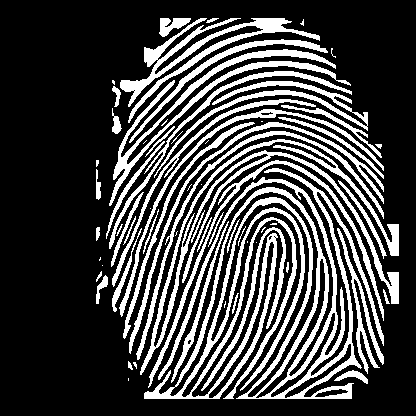
\includegraphics[width=0.25\linewidth]{obrazky-figures/eval_results/optical_gabor.png}\hfill
    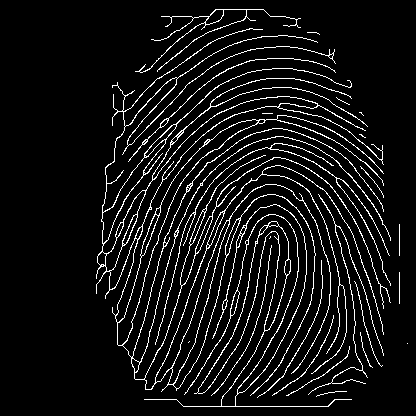
\includegraphics[width=0.25\linewidth]{obrazky-figures/eval_results/optical_thin.png}\hfill
    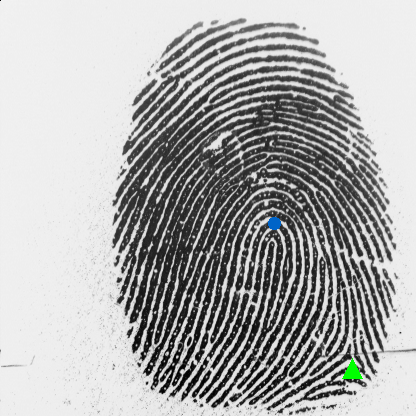
\includegraphics[width=0.25\linewidth]{obrazky-figures/eval_results/optical_singularities.png}
    \caption{Výsledky spracovania snímok z optického snímača.}
    \label{obr:vyhodnotenie_optical}
  \end{figure*}

  \begin{figure*}[h]\centering
    \centering
    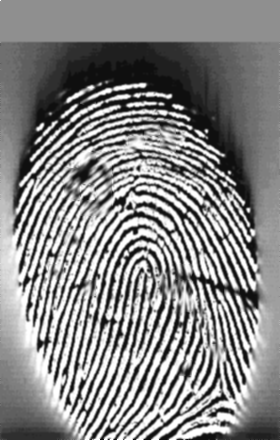
\includegraphics[width=0.25\linewidth]{obrazky-figures/eval_results/termal_orig.png}\hfill
    
\includegraphics[width=0.25\linewidth]{obrazky-figures/eval_results/termal_freq.png}\hfill
    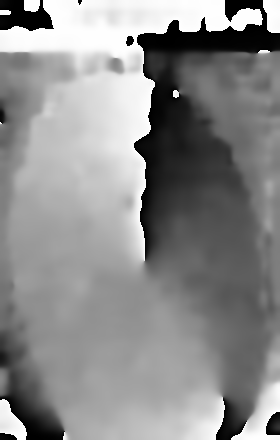
\includegraphics[width=0.25\linewidth]{obrazky-figures/eval_results/termal_orient.png}
    \\[1pt]
    
\includegraphics[width=0.25\linewidth]{obrazky-figures/eval_results/termal_gabor.png}\hfill
    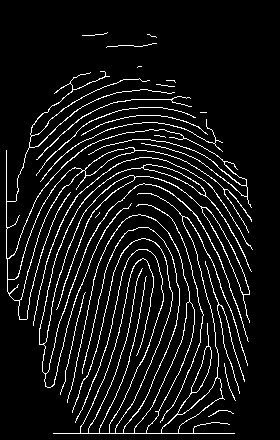
\includegraphics[width=0.25\linewidth]{obrazky-figures/eval_results/termal_thin.png}\hfill
    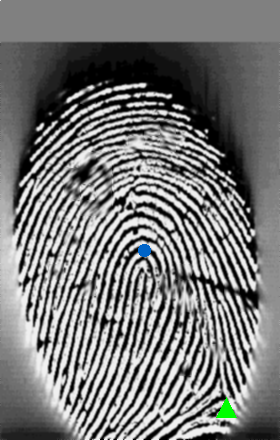
\includegraphics[width=0.25\linewidth]{obrazky-figures/eval_results/termal_singularities.png}
    \caption{Výsledky spracovania snímok z termálneho snímača.}
    \label{obr:vyhodnotenie_termal}
  \end{figure*}

  \begin{figure*}[h]\centering
    \centering
    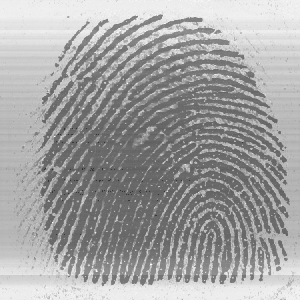
\includegraphics[width=0.25\linewidth]{obrazky-figures/eval_results/capac_orig.png}\hfill
    
\includegraphics[width=0.25\linewidth]{obrazky-figures/eval_results/capac_freq.png}\hfill
    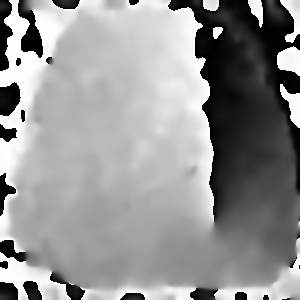
\includegraphics[width=0.25\linewidth]{obrazky-figures/eval_results/capac_orient.png}
    \\[1pt]
    
\includegraphics[width=0.25\linewidth]{obrazky-figures/eval_results/capac_gabor.png}\hfill
    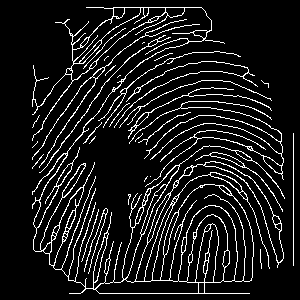
\includegraphics[width=0.25\linewidth]{obrazky-figures/eval_results/capac_thin.png}\hfill
    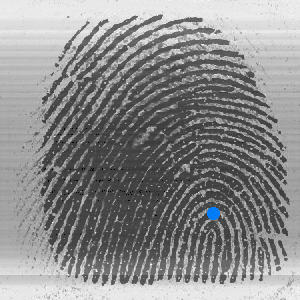
\includegraphics[width=0.25\linewidth]{obrazky-figures/eval_results/capac_singularities.png}
    \caption{Výsledky spracovania snímok z kapacitného snímača.}
    \label{obr:vyhodnotenie_capac}
  \end{figure*}

% Umístění obsahu paměťového média do příloh je vhodné konzultovat s vedoucím
%\chapter{Obsah přiloženého paměťového média}

%\chapter{Manuál}

%\chapter{Konfigurační soubor}

%\chapter{RelaxNG Schéma konfiguračního souboru}

%\chapter{Plakát}

% //TODO prilohy